\documentclass{article}
\usepackage[utf8]{inputenc}
\usepackage{listings}
\usepackage{cite}
\usepackage{amsmath,amssymb,amsfonts}
\usepackage{algorithmic}
\usepackage{graphicx}
\usepackage{textcomp}
\usepackage{xcolor}
\usepackage{color}
\usepackage{url}
\usepackage[parfill]{parskip}
\definecolor{dkgreen}{rgb}{0,0.6,0}
\definecolor{gray}{rgb}{0.5,0.5,0.5}
\definecolor{mauve}{rgb}{0.58,0,0.82}
\lstset{%
    aboveskip=3mm, belowskip=3mm,
    showstringspaces=false,
    columns=flexible,
    basicstyle={\small\ttfamily},
    numbers=none,
    numberstyle=\tiny\color{red},
    keywordstyle=\color{blue},
    commentstyle=\color{dkgreen},
    stringstyle=\color{mauve},
    breaklines=true,
    breakatwhitespace=true,
    tabsize=3
}

\newcommand{\code}[1]{\texttt{#1}}
\newcommand{\val}[1]{#1_{\text{val}}}
\newcommand{\est}[1]{#1_{\text{est}}}

\begin{document}
\title{Lab 2 --- Boosting}
\author{Malcolm Vigren, \textit{malvi108} \\
        Emil Segerbäck, \textit{emise935}}

\maketitle

\section{Classification accuracy}

A plot of the accuracies for the training and testing is shown in Figure~\ref{fig:acc}.

\begin{figure}[h]
  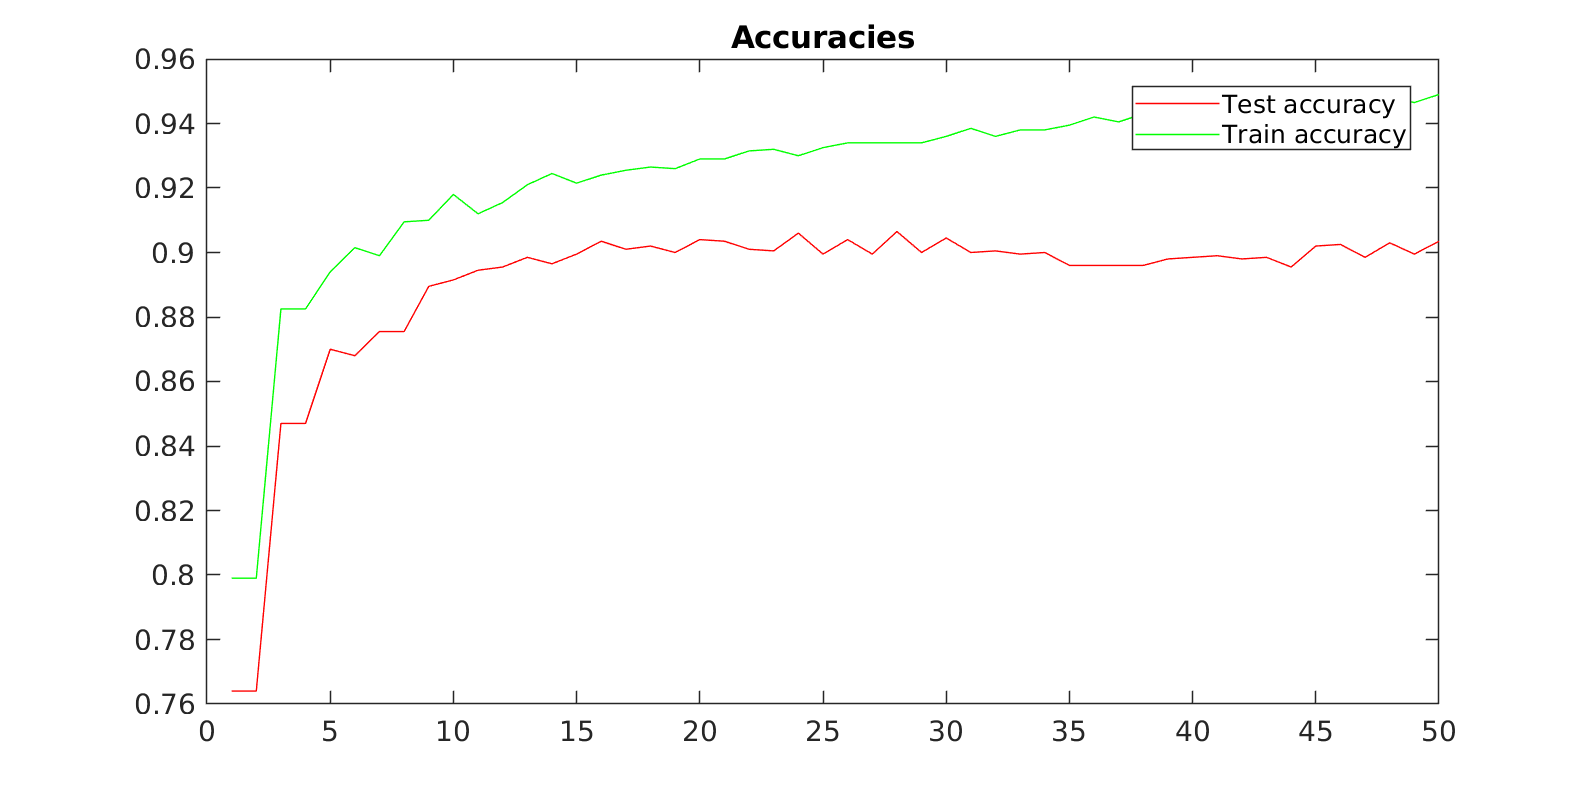
\includegraphics[width=13cm]{accuracies.png}
  \caption{Accuracies for classifying test and training data}
  \label{fig:acc}
\end{figure}

\section{Weak classifiers}

We used 50 weak classifiers when training. 25 weak classifiers were
used in the strong classifier, since the test accuracy did not further
improve with more classifiers, as shown in Figure~\ref{fig:acc}.

Our strong classifier seemed to get an accuracy of about 90\%.

\begin{figure}[h]
  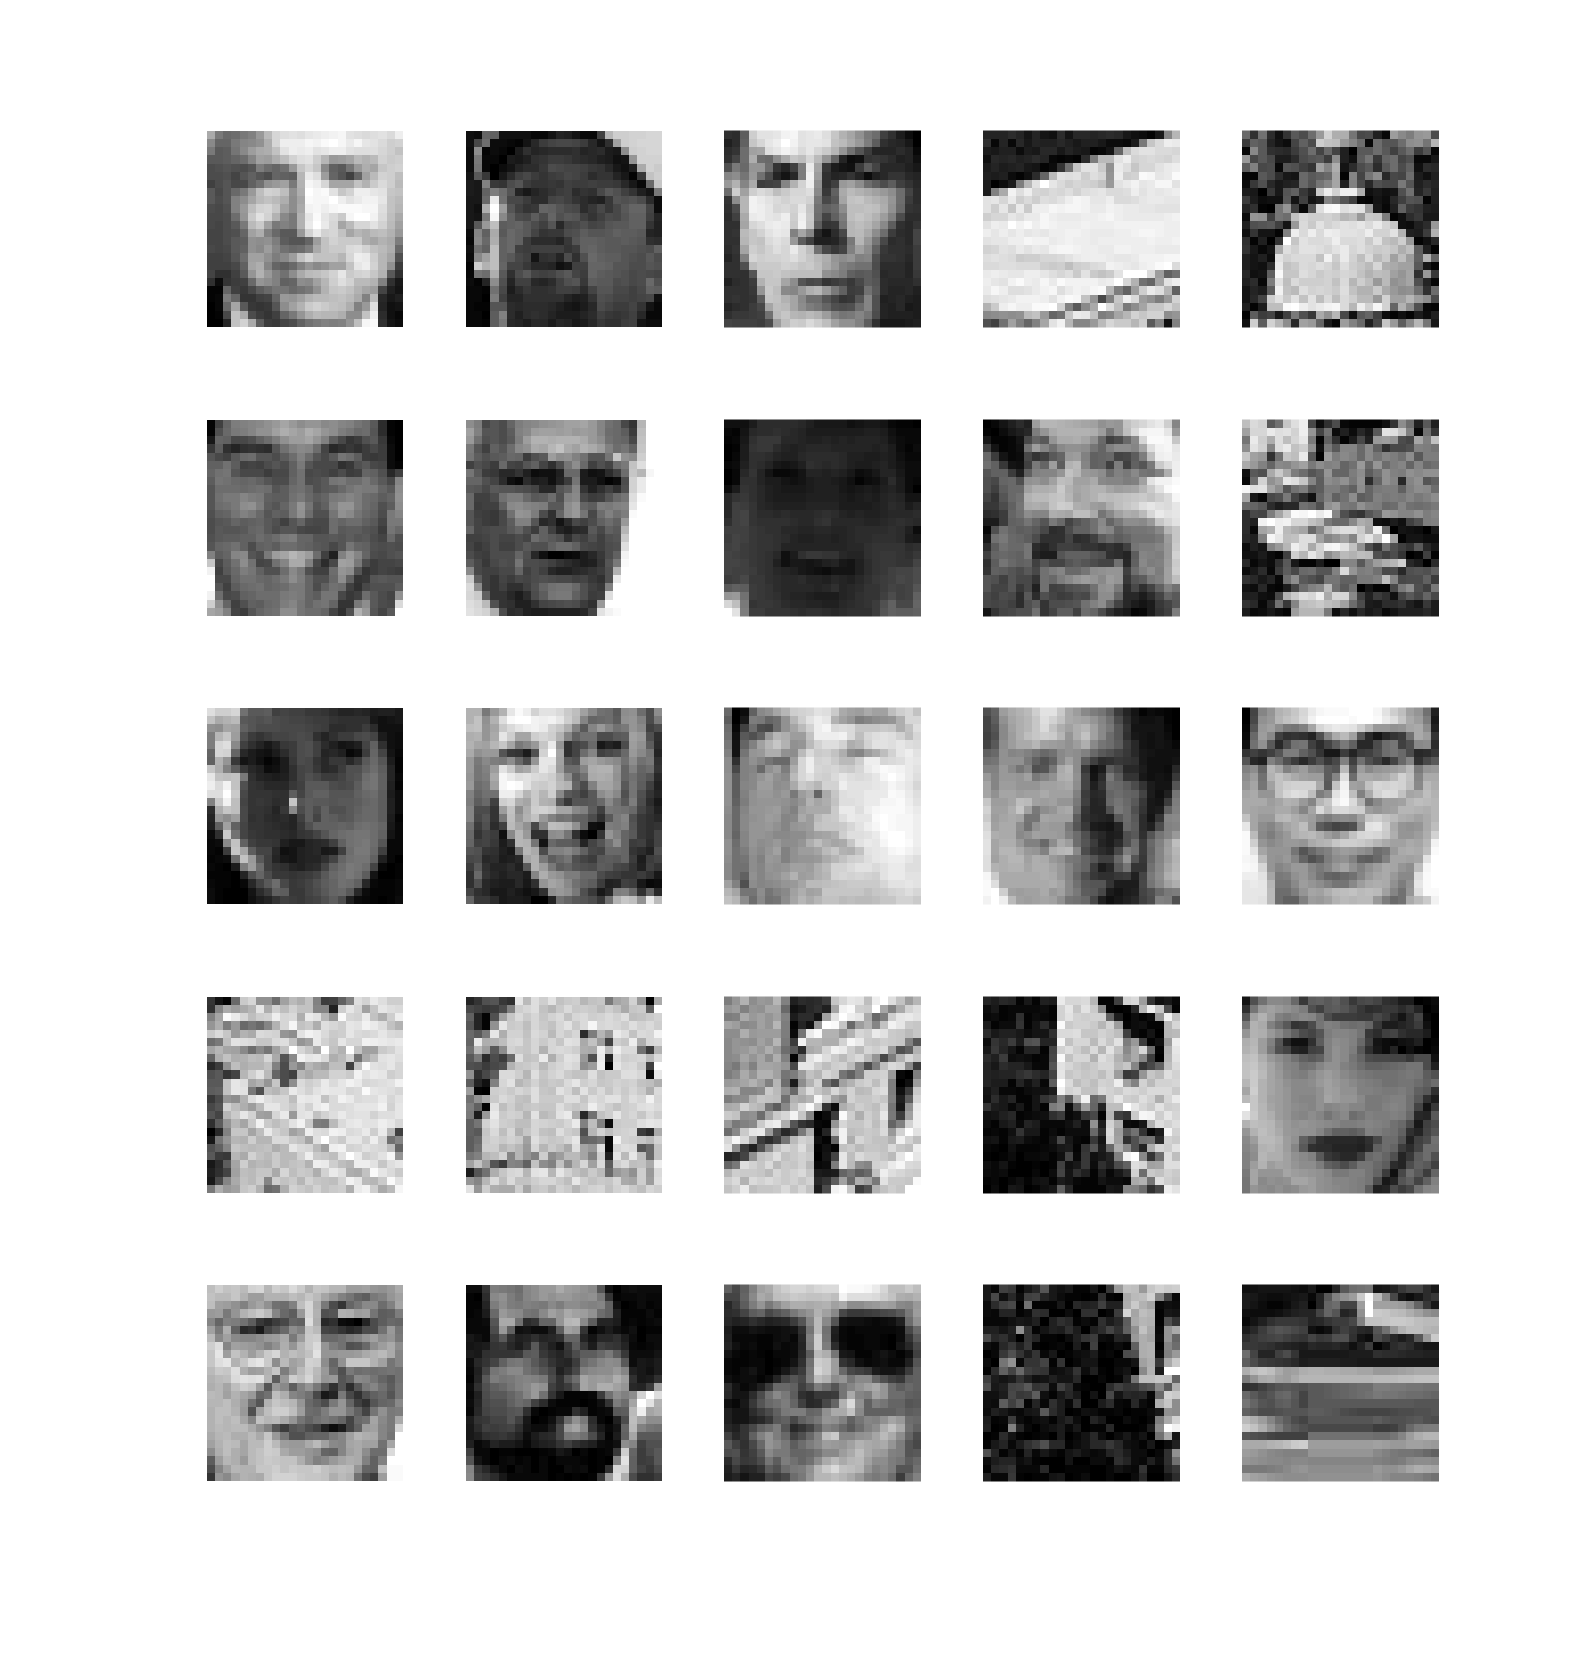
\includegraphics[width=10cm]{faces.png}
  \caption{Faces and non-faces that were incorrectly classified}
  \label{fig:faces}
\end{figure}

In Figure~\ref{fig:faces} there are 25 images that were incorrectly
classified. We can see that some of the faces that were not classified
as such have poor contrast or uncommon facial expressions. There are
some images though that we cannot quite understand why they were not
correctly classified.

We can never expect perfect results because magic is not possible.

\end{document}
